\documentclass[UTF8]{ctexart}
\usepackage{amsmath, amsthm, amssymb, graphicx, amsfonts, indentfirst}
\usepackage{fancyhdr,color,framed,enumitem,tocloft}
\usepackage{subcaption}
\usepackage{algorithm}
\usepackage{algorithmic}
\usepackage{booktabs}
\usepackage{multicol}
% \usepackage{subfigure}
\usepackage[perpage]{footmisc}
\linespread{1.5}
\usepackage[letterpaper,top=2cm,bottom=2cm,left=3cm,right=3cm,marginparwidth=1.75cm]{geometry}
\usepackage[colorlinks,
            linkcolor=blue,
            anchorcolor=blue,
            citecolor=blue]{hyperref}

%\ctexset{subsubsection = {number=\arabic{subsubsection}}}       %subsubsection形式改为1,2,3,...
\title{大数据分析计算机基础期末作业}
\date{\today}
\author{李健宁\thanks{李健宁,2401210081,数学科学学院}}
\setlength{\parindent}{4pt}
\setlength{\headheight}{27pt}
\pagestyle{fancy}

\setlength{\cftbeforesecskip}{0.5\baselineskip} 
\begin{document}
\maketitle

\tableofcontents

\clearpage

\section{项目结构}

\begin{itemize}[itemsep=0pt,topsep=0pt]
    \item \texttt{truckGps.ipynb} 货车GPS数据分析的源代码;
    \item \texttt{项目总结报告.pdf} 本文件,对整个项目的汇总和说明;
    \item \texttt{sample1.csv} 原数据文件前500000行的样本,用以预处理数据,未被包含在本次提交的文件中;
    \item \texttt{E://20170906.csv} 货车GPS数据,未被包含在本次提交的文件中;
    \item \texttt{./output} 部分中间结果的存储,未被包含在本次提交的文件中;
    \item ./html 数据点映射到路网数据的描点图:
        \begin{itemize} [itemsep=0pt,topsep=0pt]
            \item \texttt{Top20.html} 最密聚集地前20名位置图;
            \item \texttt{Top20withOD.html} 最密聚集地前20名位置图和目的地、出发地前20名位置图;
            \item \texttt{重叠.html} 未采取区域去重时的前20名最密聚集地位置图;
        \end{itemize}   
    \item \texttt{./img} 项目总结报告中需要的图片或可视化结果;
        \begin{itemize}[itemsep=0pt,topsep=0pt]
            \item \texttt{./pre} 预处理数据的辅助图片,均在本文件中引用;
            \item \texttt{./时序分析}  20个最密聚集地的进入时间和离开时间的时序分析,以及总体的进入时间和离开时间的时序分析;
            \item \texttt{./OD分析}\  20个最密聚集地的OD分析结果,以及总体的OD分析结果。
            \item \texttt{*.png} 其他在本文件中使用的图片或可视化结果。
        \end{itemize}
\end{itemize}

\section{数据介绍}

数据为货车 GPS 数据。原数据共包含$67490000$ 条数据,每条数据共8列,前四列依次为脱敏车号、日期时间和经纬度(占两列)。数据的地理范围大致在北京市内,共涉及车辆$74578$ 辆。进行初步分析时,我们使用原数据的前$500000$条数据。

\section{数据清洗和整理}

由于部分列名未定,我们需要同时进行清洗与整理工作,每当确定一部分列名,便可以根据列名的性质清理掉不符合要求的数据,进一步辅助后续列名的判断。

本部分数据分析借助了VS code的Data Wrangler的插件,能够对海量数据进行可视化及快速的数据筛选排序,并自动展示每列的统计信息,在确定列名时非常好用。

\subsection{确定列名}

已知第3、4列为经纬度,我们清洗掉经纬度范围不在北京市范围内的所有数据,我们无法利用这些数据,且这些数据也通常伴随着不正常的时间戳。

北京经度大约在$115.41°E$至$117.51°E$之间,纬度大约在$39.44°N$至$41.06°N$之间,我们将有效数据的经纬度限定在$[115.41°,117.51°]E\times [39.44°, 41.06°]N$。这部分清理了$121987$条数据。

本部分数据清除后,第7列数据的分布(图\ref{7-stat})非常清晰,数据范围为$[0,360]$中的整数,除去数值为$0$的数据后近似均匀分布,不过在$90$的整倍数所在的分布区间有峰值,基本符合北京市南北向和东西向道路居多,其他方向道路兼而有之的特点。我们猜测这列数据是货车的行驶方向。进一步我们取出某个车号,观察该辆车所有的数据信息(图\ref{v}),我们发现此列数据连续性较大,进一步印证了我们的猜测。

\begin{figure}[!htb]
    \centering
    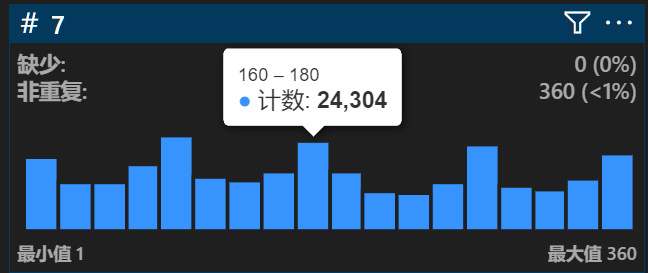
\includegraphics[width = 0.6\textwidth]{../img/pre/7列统计信息.png}
    \caption{根据经纬度清理后第7列统计信息}
    \label{7-stat}
\end{figure}

除此之外,我们发现根据车号分组后有部分重复信息,因此去除重复的行,这部分清理了$14219$条数据。这可能是为了避免GPS信号未正常接收采取的数据冗余策略,但清理掉的数据占比较小,这一猜测或许并不靠谱。

进一步观察第5列的数据分布,最大值为123,除去数值为$0$的数据后数据分布如图\ref{4-stat},速度在80以下的占比较高,超过80的数据量较小,但在$[100,120]$范围内仍有相当数量的数据。因此我们猜测此列是速度信息,在非高速路段速度在$80$以下,高速路段速度在$[100,120]$(和现实中货车高速限速$100$或$110$以及存在小幅度超速现象是相符合的)。进一步我们取出某个车号,观察该辆车所有的数据信息(图\ref{v}),我们发现此列数据连续性较大,进一步印证了我们的猜测。这一信息可以通过将该列数据根据经纬度映射到地图后和高速路段、非高速路段上的分布进行验证。

\begin{figure}[!htb]
    \centering
    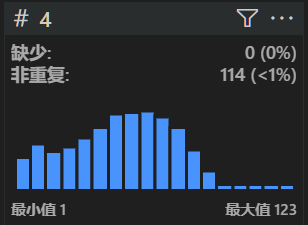
\includegraphics[width = 0.4\textwidth]{../img/pre/4列统计信息.png}
    \caption{第4列统计信息}
    \label{4-stat}
\end{figure}

\begin{figure}[!htb]
    \centering
    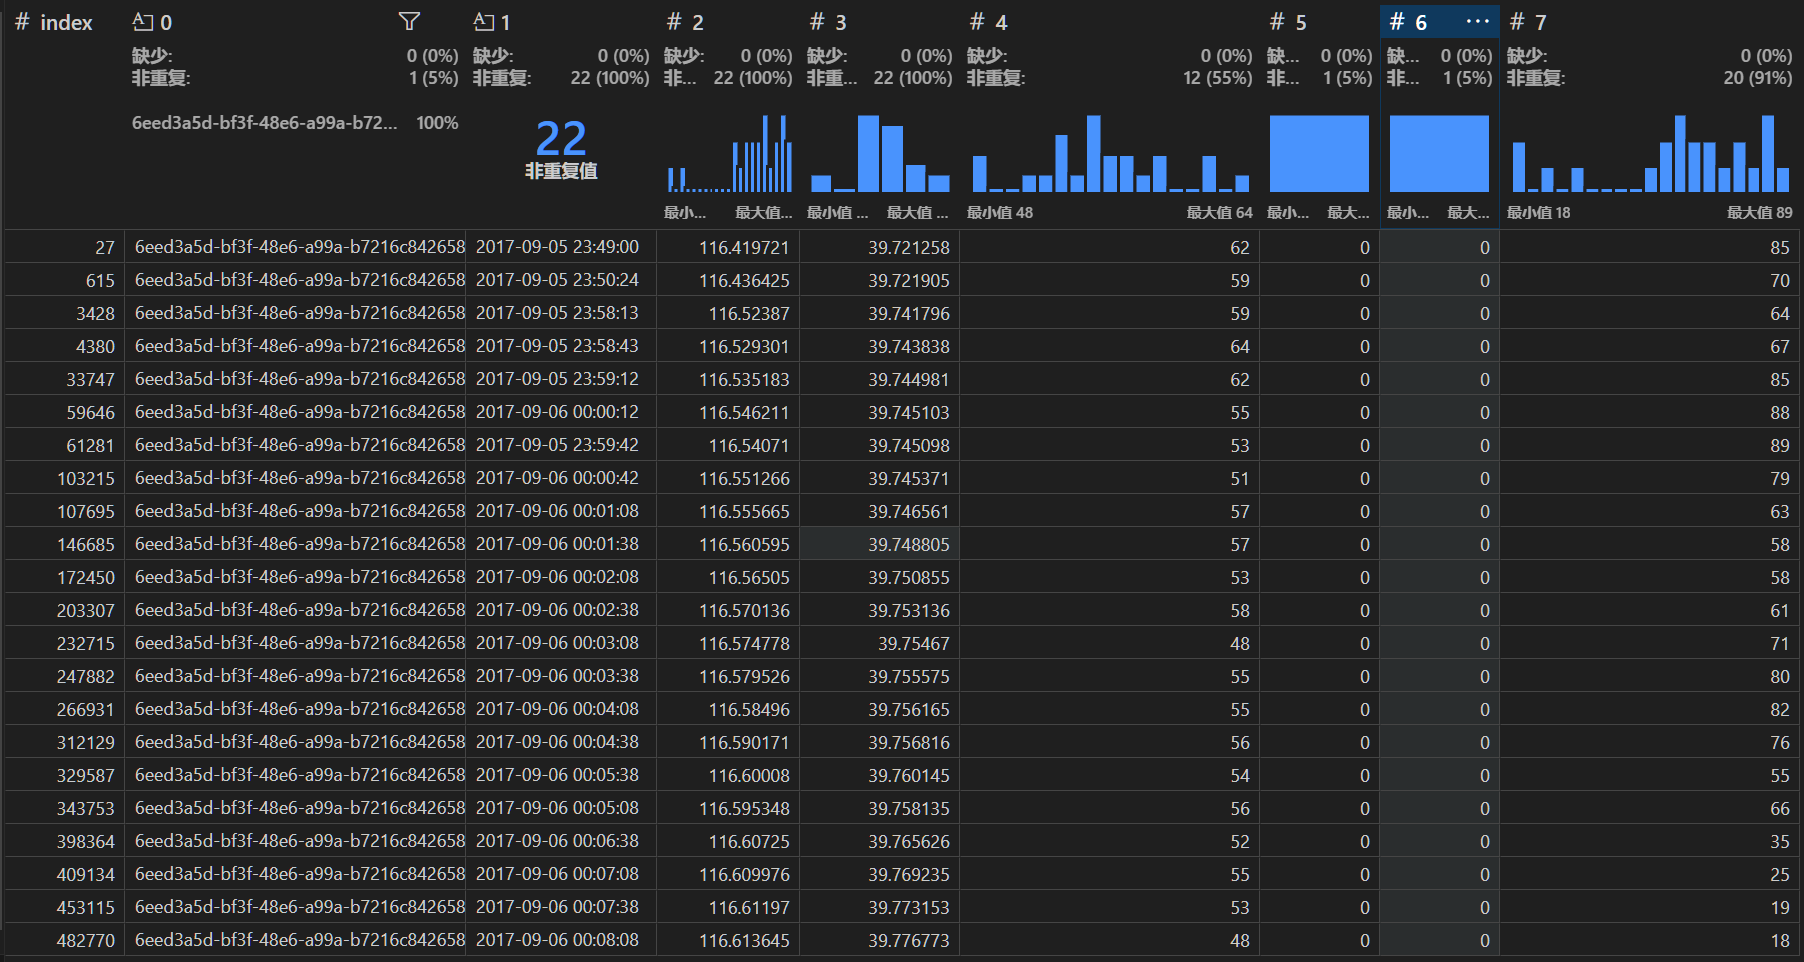
\includegraphics[width = 0.9\textwidth]{../img/pre/速度推断信息.png}
    \caption{某辆车的数据总览和统计信息}
    \label{v}
\end{figure}

此时仍然剩余两列的列名未知,根据车号分组发现第5列数据在很多位置上和第4列相差很小,$33607$辆车中,只有$845$辆车的第6列数据存在两个或以上的值,其余$97.5\%$的车辆第6列的值是固定的,另一方面只有$1197$辆车的第6列数据中存在$1$,因此这一列的信息量并不大。至此,我们忽略这两列数据。

结合网络查找的资料\href{https://www.heywhale.com/mw/dataset/5f75ad252b83e00030b3f91d/file}{150万条营运车辆GPS数据}中对于每项数据的数据分布和统计信息,能够进一步印证关于速度和行驶方向这两列列名的猜测是正确的。

\subsection{数据清洗}

清除时间戳不在2017年9月5-6日的数据,清除数据$1367$条,剩余$33437$辆车的$362427$条数据。我们将上述流程分别应用于$100000$条数据和$1000000$条数据以及全量数据,每次清理和保留的数据的比例大致相当,因此我们可以认为这些数据清理流程是合理的。

表\ref{data}给出对于不同数据规模下每部分清理的数据和保留的数据的数量和所占的比例。
\begin{table}[ht]
    \begin{center}
        \caption{数据清洗统计表}
        \label{data}
    \begin{minipage}{\textwidth}
    \centering
    \begin{tabular}{r|l|l|l|l}
        \hline \hline
    \textbf{数据量} & \textbf{100000} & \textbf{500000} & \textbf{1000000} & \textbf{67490000} \\ \hline
    车辆数 & 35017 & 43955 & 44923 & 74578 \\ \hline \hline
    经纬度清洗数量 & 27357 & 121987 & 239879 & 15911169 \\ \hline 
    剩余数据 & 72643 & 378013 & 760121 & 51578831 \\ \hline
    经纬度清洗比例\footnote{比例指当前阶段清洗数量占上一阶段剩余数据的比例,除最后一行的剩余数据比例指剩余数据占初始数据量的比例外,下同。} & 27.36\% & 24.40\% & 23.99\% & 23.58\% \\ \hline \hline
    重复数据清洗 & 2320 & 14219 & 28073 & 1879882 \\ \hline
    剩余数据 & 70323 & 363794 & 732048 & 49698949 \\ \hline
    重复数据清洗比例 & 3.19\% & 3.76\% & 3.69\% & 3.64\% \\ \hline \hline
    时间戳清洗 & 286 & 1367 & 2745 & 221973 \\ \hline
    剩余数据 & 70037 & 362427 & 729303 & 49476976 \\ \hline
    时间戳清洗比例 & 0.41\% & 0.38\% & 0.37\% & 0.45\% \\ \hline \hline
    停车数据清洗 & 48248 & 251557 & 507017 & 34059171 \\ \hline
    剩余数据 & 21789 & 110870 & 222286 & 15417805 \\ \hline
    停车数据清洗比例 & 68.89\% & 69.41\% & 69.52\% & 68.84\% \\ \hline \hline
    剩余车辆 & 6454 & 8377 & 9873 & 57693 \\ \hline
    剩余数据 & 21789 & 110870 & 222286 & 15417805 \\ \hline
    剩余数据比例 & 21.79\% & 22.17\% & 22.23\% & 22.84\% \\ 
    \hline \hline
    \end{tabular}
    \end{minipage}    

    \end{center}
    \end{table}

\section{聚集地计算}

本节我们着手寻找货车前20名聚集地,并进行可视化。

\subsection{前20名聚集地}

同样的,我们先对要寻找的聚集地做一些假设。

\subsubsection{近似正方形和经纬度上间隔$1km$}

我们假定1平方公里范围的区域是约$1km\times 1km$的近似正方形,每条边分别与一条经线或纬线重合。根据北京市的经纬度范围,我们近似的认为上述近似正方形是纬度相差$\text{grid\_lat} = 0.0089927^\circ$,经度相差$\text{grid\_lon} = 0.011723^\circ$的四条经纬线围围成的。这两个数值是我们使用北京市中心的经纬度$39.906217°N, 116.3912757°E$分别向北和东走1km后变化的纬度和经度得到的。在北京市域小范围内,我们粗略的认为纬度变化引起的距离变化可以忽略不计。

至此,我们的目标已经转换为寻找前述的近似正方形。

\subsubsection{回顾}

我们先回忆一下之前寻找最密区域的算法\ref{alg-1}。我们希望采取类似的算法计算最密聚集地。

\begin{algorithm}[htb]
    \caption{寻找数据最多的 1 平方公里区域}
    \label{alg-1}
    \begin{algorithmic}[1]
    \STATE \textbf{Input:} 数据点集合 \texttt{df},经度和纬度的间隔 \texttt{grid\_lat, grid\_lon},阈值 $\alpha$
    \STATE \textbf{Output:} 数据最密区域 $R$,区域 $R$ 点个数 $n$
    \STATE 将北京市经纬度按照 \texttt{grid\_lat, grid\_lon} 划分为若干段
    \STATE \texttt{grid\_count},表示一个 $2km \times 2km$ 的区域中数据点的个数
    \FOR{point \textbf{in} \texttt{df}}
        \STATE 找到 point 所处的纬度和经度的坐标 \texttt{[lat\_idx, lon\_idx]}
        \STATE 为它所在的 $4$ 个 $2km \times 2km$ 区域的 \texttt{grid\_count += 1} 
    \ENDFOR
    \STATE 选择 \texttt{grid\_count} 中数据点最多的区域作为\texttt{参考区域}
    \FORALL{以 $100m$ 为步长的 $121$ 个 $1km \times 1km$ 区域}
        \STATE 找出点数最多的小区域 $R$ 和点数 $n$
    \ENDFOR
    \STATE 计算 $n$ 占总数据的比例 $\beta = \frac{n}{\sum_{grid\_count}}$
    \STATE 搜索 \texttt{grid\_count} 中占总数据量的比例大于 $\beta$ 的 $2km \times 2km$ 区域,得到若干个 \texttt{备选区域}
    \FOR{每个 \texttt{备选区域}}
        \FORALL{以 $100m$ 为步长的 $121$ 个 $1km \times 1km$ 区域}
            \STATE 找出点数最多的小区域 $R_1$ 和点数 $n_1$
        \ENDFOR
    \ENDFOR
    \RETURN $R_1$, $n_1$
    \end{algorithmic}
\end{algorithm}

\subsubsection{尝试}\label{try}

首先需要注意的是,我们这里要求的聚集地,和第三次作业中的最密区域定义略有不同。聚集地偏向于车辆的聚集程度,对于\textbf{同一辆车在某个区域内的多条数据,我们应该只计数一次}。

不过,这样就无法区分一辆车在一天之内多次到达某个区域的情况,因此我们需要对同一辆车的数据进行处理,如过两条数据的时间戳相差不超过$30$分钟,我们认为这是同一次行程,只计数一次;如果相差超过$30$分钟,我们认为这是两次行程,计数两次。

在具体的实现上,先对数据按照车号、时间戳两列排序,之后维护一个时间戳的字典,每当有数据进入某一区域,如果车号不在字典中,或车号对应的时间戳超过$30$分钟,更新时间戳,计数加一;否则忽略这条数据。不过这种方法的问题在于,我们需要为每个区域维护一个车号:时间戳的字典,空间复杂度是$O(n)$,不适合大规模数据的处理。

存在的另一个显著问题是,如果我们使用之前清洗过的所有数据,那么计算出的聚集地均是\textbf{复杂立交桥所在的区域}(图\ref{bridge}),这有可能是因为我们所寻找的区域形状和常见的复杂立交桥的尺度相近,这与我们希望找到的聚集地是明显不符的。

\begin{figure}[!htb]
    \centering
    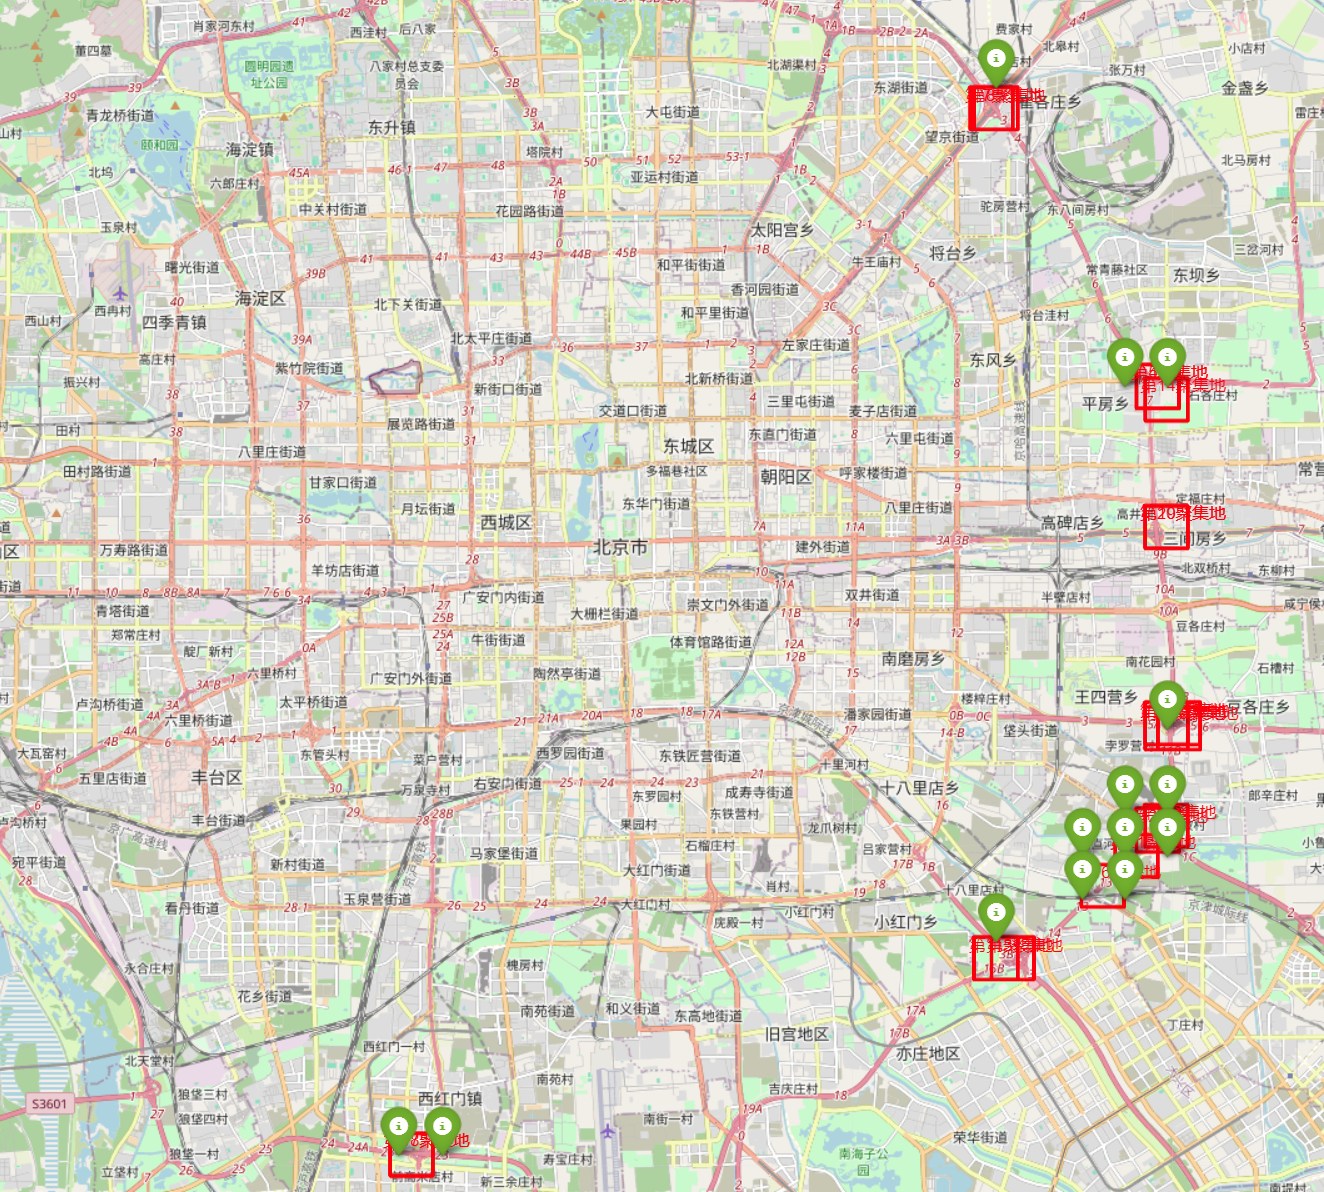
\includegraphics[width = \textwidth]{../img/立交桥.png}
    \caption{最密聚集地常出现在复杂立交桥所在区域}
    \label{bridge}    
\end{figure}

为了解决以上问题,我们最终选择只使用静止数据,并扩大区域范围的方法。静止数据相较于车辆的行驶轨迹更能反映车辆的聚集程度。在计算OD时算法和使用所有数据类似,而且静止数据的特征使得判断进入时间、离开时间更加方便,这些在后续内容中将详细介绍。

另一方面,我们将区域范围扩大到$2km\times 2km$,这降低了立交桥对整个区域的影响。

\subsubsection{算法}

在数据上,只保留速度$v>2$的数据;在变换区域尺度上,我们只需要将先前的\texttt{grid\_lat, grid\_lon}分别乘2即可。在算法上,由于我们现在要求前20名,我们先对所有的大区域进行计数排序,取前20名的区域作为参考区域,分别计算每个参考区域的最密子区域,得到20个最密子区域的最小值作为阈值$\beta$\footnote{这里我们不再采取占总数据点的比例(因为这是一个常数,我们只需比较值的大小即可。};再次搜索所有的大区域,找到点数超过$\beta$的区域作为备选区域,分别计算备选区域的最密子区域后取前20名,这些区域就是我们要找的聚集地前20名\footnote{在误差$200m$范围内的前20名,因为事实上我们找到了所有数据点超过第20名小区域的大区域,并且遍历了这些大区域中的小区域。}。

不过由于我们只取了每个大区域中的最密子区域,当部分大区域中存在多个数据点很多的小区域时,可能会出现遗漏;对于某些区域会出现多个前20名聚集地并有很多重叠(如图\ref{重叠}。比如新发地附近的区域占据了前20名多个区域)。这主要是因为部分市场、货场等占地面积较大,覆盖了多个大区域,而大区域相互之间存在重叠。

\begin{figure}[!htb]
    \centering
    \begin{minipage}{\textwidth}
        \centering
        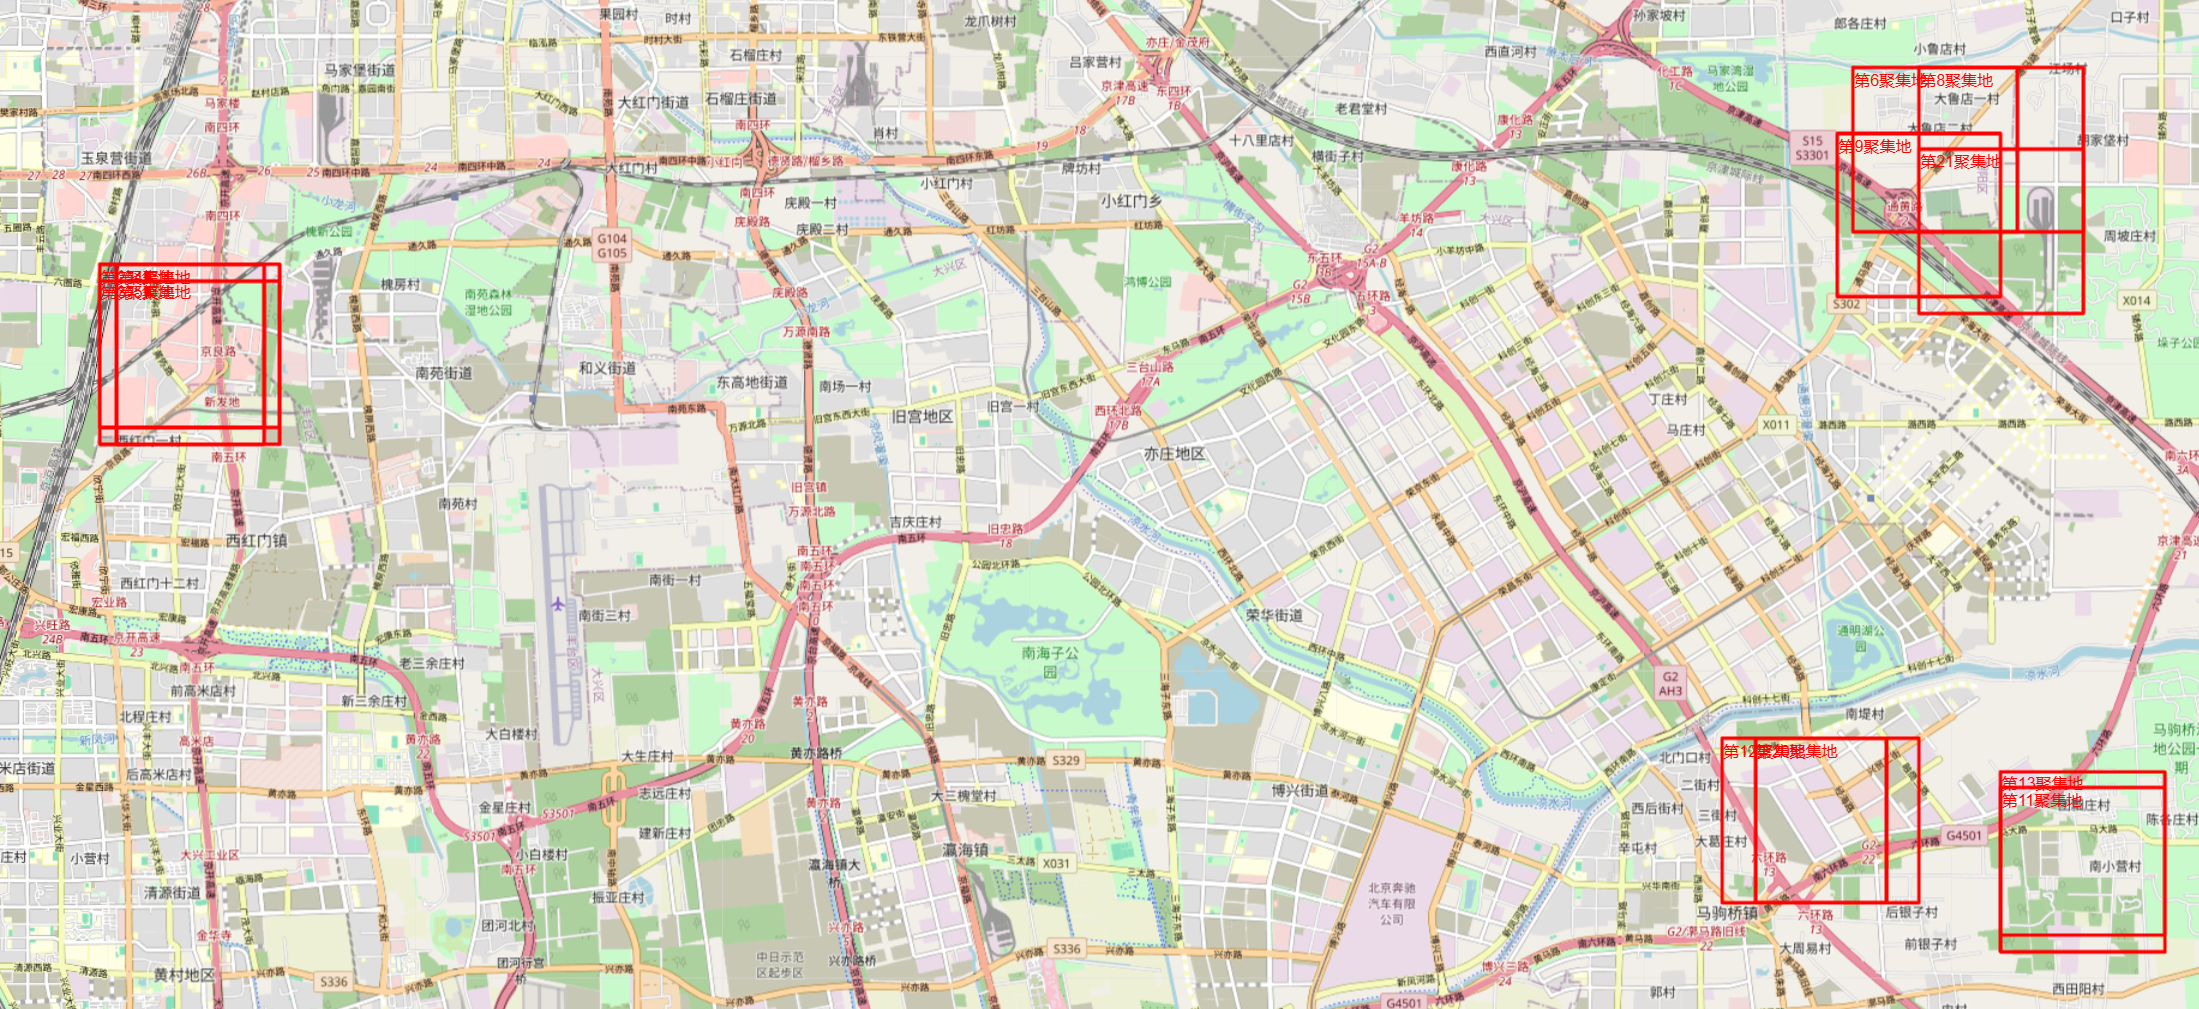
\includegraphics[width=\textwidth]{../img/重叠.png}
        \caption{区域重叠}
        \label{重叠}
    \end{minipage}
    \begin{minipage}{\textwidth}
        \footnotesize % 调整脚注文字大小
        \textbf{注:} 截取自\texttt{./html/重叠.html}。 % 这里是脚注内容
    \end{minipage}
\end{figure}

% #TODO \footnotemark
% \footnotetext{截取自\texttt{./html/重叠.html}。}

\begin{figure}
    \centering
    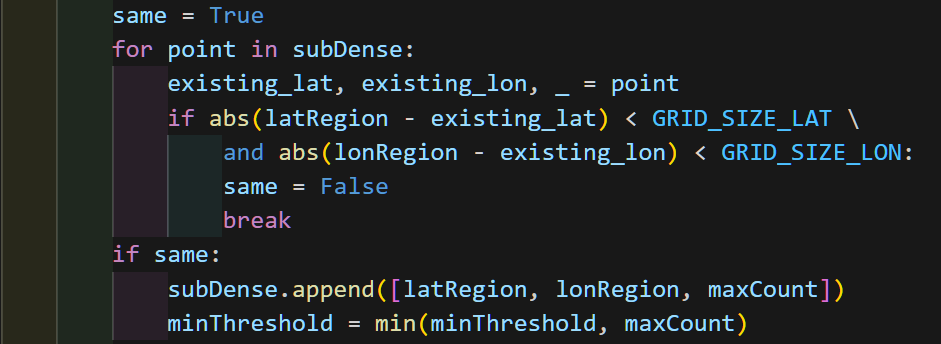
\includegraphics[width = \textwidth]{../img/去重代码.png}
    \caption{去除重复聚集地区域的代码}
    \label{去重code}
\end{figure}

\paragraph{区域重叠} 为了解决区域重叠的问题,我们在取最密聚集地前20名时,依次判断新加入的区域和已有的区域是否存在重叠,如果存在,我们舍弃当前区域继续取下一个(图\ref{去重code})。这样便能够获得更多聚集地的信息(图\ref{drop})。根据我们取的顺序,也能够保证数据点多的区域排名更靠前。自然地,我们也无需再考虑子区域遗漏的问题。

\begin{figure}[htb]
    \centering
    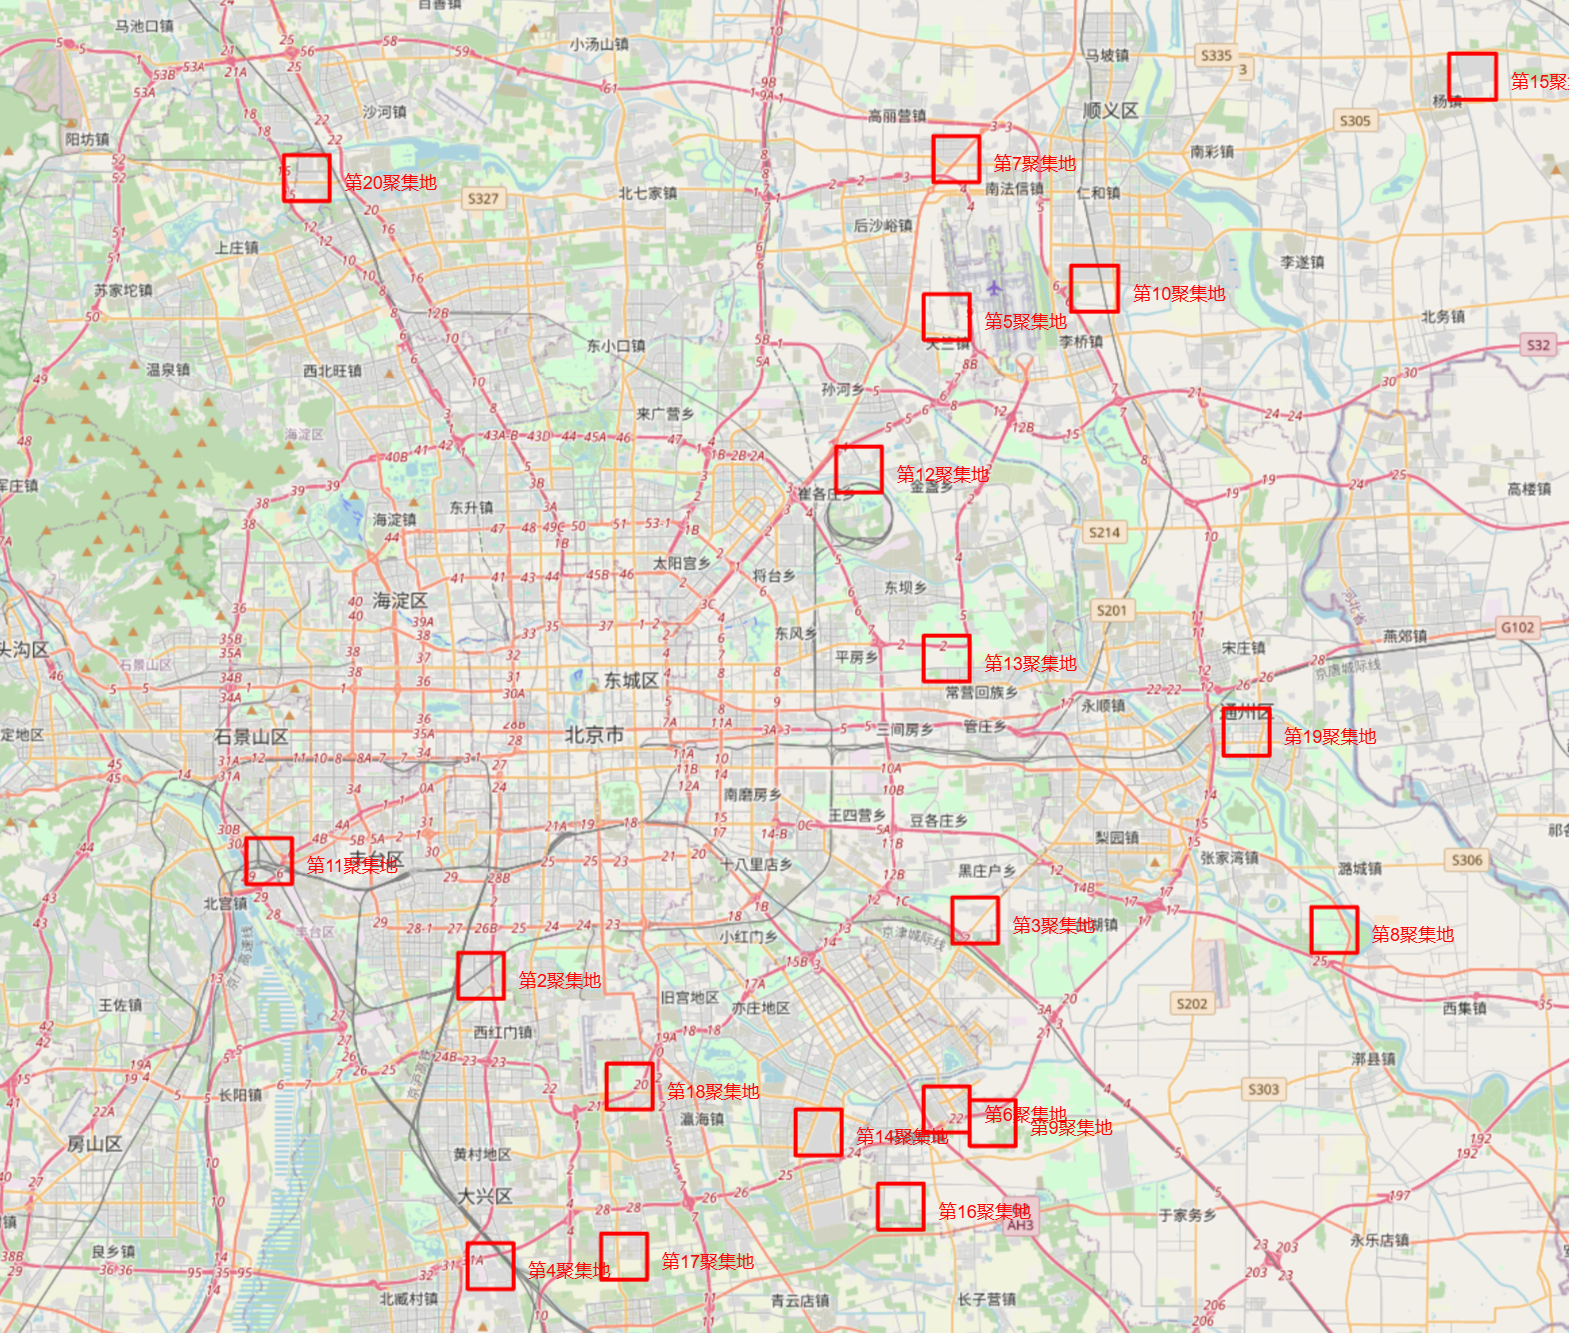
\includegraphics[width = \textwidth]{../img/去重.png}
    \caption{去除重复区域后最密聚集地的概览,$n=500000$}
    \label{drop}
\end{figure}

\paragraph{数据点去重} 我们还需要处理之前提到过的数据点去重的问题。在\ref{try}中我们希望通过时间间隔来计算,但采取字典会导致空间复杂度过高。经过思考后我们能发现两个关键事实\textbf{需要去重的点来自相同的车辆;每辆车辆的数据点个数并不多}。在这种假设下,我们首先根据车号分组,在组内根据时间排序。在排序后,我们只需要维护一个滑动窗口,表示过去若干条数据的位置,就可以在$O(window)$的时间\footnote{判断点是否在窗口内和窗口弹出操作的复杂度都是$O(window)$。我们还尝试了利用双端队列和哈希表来实现滑动窗口以期降低这两个操作的时间复杂度,但这会带来空间复杂度的显著提升,且时间上的提升也并不明显,最终仍然采用列表实现滑动窗口。}内判断当前数据点是否需要计数\footnote{通过调整窗口大小也能够调整去重的范围,窗口越长,计数两次的时间点就需要间隔越长时间。},为了后续统计方便,我们在\texttt{Dataframe}中增加一列\texttt{valid}表示数据有效。这种方法的空间复杂度是$O(window)$\footnote{只需要维护一个滑动窗口。},更适合大规模数据的处理。

\begin{algorithm}[htb]
    \caption{寻找最密聚集地前20名}
    \label{alg-2}
    \begin{algorithmic}[1]
    \STATE \textbf{Input:} 静止数据点集合 \texttt{df},经度和纬度的间隔 \texttt{grid\_lat, grid\_lon}
    \STATE \textbf{Output:} 数据最密区域和计数 {Top20}
    \STATE 将北京市经纬度按照 \texttt{grid\_lat, grid\_lon} 划分为若干段
    \STATE 初始化二维列表 \texttt{grid\_count},表示一个 $4km \times 4km$ 的区域中数据点的个数
    \FOR{point \textbf{in} \texttt{df}}
        \STATE 找到 point 所处的纬度和经度的坐标 \texttt{[lat\_idx, lon\_idx]}
        \STATE 为它所在的 $4$ 个 $4km \times 4km$ 区域的 \texttt{grid\_count += 1} 
    \ENDFOR
    \STATE 选择 \texttt{grid\_count} 中前20名的区域作为\texttt{参考区域}
    \FOR{区域$ref_k$ \textbf{in} \texttt{参考区域}}
        \FORALL{$200m$为步长的 $121$ 个 $2km \times 2km$ 区域}
            \STATE 找出$ref_k$中点数最多的小区域 $R_k$ 和点数 $n_k$
        \ENDFOR
    \ENDFOR
    \STATE  计算阈值 $\beta = \min_{k}{n_k}$
    \STATE 搜索 \texttt{grid\_count} 中大于 $\beta$ 的 $4km \times 4km$ 区域,得到若干个 \texttt{备选区域}
    \FOR{区域$cand_k$ \textbf{in} \texttt{备选区域}}
        \FORALL{$200m$ 为步长的 $121$ 个 $2km \times 2km$ 区域}
            \STATE 找出$cand_k$中点数最多的小区域 $R_k$ 和点数 $n_k$,加入\texttt{Top20}
        \ENDFOR
    \ENDFOR
    \RETURN \texttt{Top20.sort()[:20]}
    \end{algorithmic}
\end{algorithm}

\subsection{结果展示}

根据算法\ref{alg-2},使用全量数据后我们计算出$\beta =8699$,前20名聚集地如表\ref{denseTable}。

\begin{table}[htb]
    \centering
    \caption{前20名聚集地}
    \label{denseTable}
    \begin{minipage}{0.48\textwidth}
        \raggedleft
        \begin{tabular}{cccc}
            \toprule
            纬度\footnotemark & 经度 & 计数 & 排名\\
            \midrule
            39.746 & 116.554 & 7307 & 1\\
            39.854 & 116.685 & 7015 & 2\\
            40.334 & 116.008 & 5626 & 3\\
            40.377 & 116.074 & 5171 & 4\\
            40.111 & 116.643 & 5060 & 5\\
            39.825 & 116.580 & 4850 & 6\\
            39.812 & 116.756 & 4709 & 7\\
            40.111 & 116.601 & 4579 & 8\\
            40.436 & 116.001 & 4518 & 9\\
            39.791 & 116.512 & 4379 & 10\\
            \bottomrule
        \end{tabular}
    \end{minipage}
    \hspace{0.005\textwidth}
    \begin{minipage}{0.48\textwidth}
        \raggedright
        \begin{tabular}{cccc}
            \toprule
            纬度 & 经度 & 计数 & 排名\\
            \midrule
            40.194 & 116.202 & 4375 & 11\\
            40.080 & 116.634 & 4290 & 12\\
            39.895 & 116.702 & 4269 & 13\\
            39.683 & 116.301 & 4234 & 14\\
            39.733 & 116.491 & 4175 & 15\\
            40.098 & 116.545 & 4059 & 16\\
            40.114 & 116.571 & 4054 & 17\\
            39.710 & 116.395 & 4045 & 18\\
            40.154 & 116.613 & 3916 & 19\\
            39.629 & 116.805 & 3713 & 20\\
            \bottomrule
        \end{tabular}
    \end{minipage}
    \begin{minipage}{\textwidth}
        \footnotesize
        \vspace{2pt}
        \textbf{注:} 这里的经纬度是区域的西北顶点,代表的是以这个点为西北角的$2km \times 2km$区域。
    \end{minipage}
\end{table}

我们将前20名聚集地的区域可视化到地图中(图\ref{dense}),并标记区域位置和数据点个数。更加详细和全面的结果可以在\texttt{./html/Top20.html}中查看。不过受\texttt{folium}库的限制,无法实现根据缩放尺度动态调整标记的大小,在缩放时会出现一些重叠。

\begin{figure}[!htb]
    \centering
    \begin{minipage}{\textwidth}
        \centering
        \includegraphics[width = \textwidth]{../img/前20名聚集地.png}
        \caption{前20名聚集地部分展示}
        \label{dense}
    \end{minipage}
    \begin{minipage}{\textwidth}
        \footnotesize % 调整脚注文字大小
        \textbf{注:} 截取自\texttt{./html/Top20.html}。 % 这里是脚注内容
    \end{minipage}
\end{figure}

\subsection{结果分析}

我们能够发现,这些聚集地基本呈现明显的区域化特征。货运车辆的聚集一般来讲对应于仓库、市场、厂房等货运需求较大的地方。

首都机场区块、东南六环区块、昌平延庆区块是三个最为密集的区块。我们分析:

\begin{itemize}[leftmargin=4em,itemsep=0pt,topsep=2pt]
    \item 首都机场区块主要是由于首都机场的货运枢纽地位,使得周围区域成为货运周转中心,出现很多厂房、仓库,进而使得货车聚集;
    \item 东南六环区块一方面是由于地理位置相对较偏僻,用地成本较低,另一方面根据北京在全国的地理位置和我国的经济结构,大量货物商品从东南两方向运抵北京,在东南郊区选择合适的位置建立仓库显然是一个合适的选择;
    \item 昌平延庆区块可能是由于这一区域和张家口方向的联系,以及这一区域本身的用地成本较低。
\end{itemize}

根据这些聚集地的分布,我们可以进一步分析货车的运输路线、货物的流向等信息。根据实际情况,有意识的划分地块用途,合理规划货运枢纽位置,提高货车的运输效率,减少交通拥堵,提高城市运输效率。

除次之外,还可以根据货车聚集地的具体情况,针对性地进行城市道路建设。比如在聚集地交通路口附近设置更多的“大车转弯盲区”提示,树立有关货车通行的交通标志,拓宽道路宽度,加大路面清扫频率等。甚至可以联合高德地图等导航软件,提示货车聚集地,提醒其他车辆等等。

\section{OD分析和时序分析}

在分析出发地、目的地和进入时间、离开时间时,重新针对所有数据计算显然不是一个聪明的办法。事实上,\textbf{在第一遍统计区域格点数据时,我们可以同步进行一些标记操作}。

以下两小节的操作均为针对最密聚集地中的某一个聚集地进行的。

\subsection{时序分析}

对于进入时间,考虑到我们计数的方法是判断当前数据是否在之前的窗口出现过,那当某条数据未出现时,就是这辆车进入当前区域的时间,\texttt{valid}就能够表示当前数据的时间戳是否是进入时间。对于离开时间,我们只需要额外增加一个\textbf{未来的滑动窗口},表示未来的若干条数据,当当前数据不在未来数据中出现时,那就是这辆车离开当前区域的时间,我们增加一列\texttt{outtime}表示当前数据的时间戳是否是离开时间。

图\ref{50}是使用$n=500000$的数据计算出的所有区域的进入时间和离开时间的分布,呈现出先进入,再离开的趋势。但采取全量数据时,呈现的分布会有一些差异。我们分析这是因为数据量增大,时间尺度拉长时,\textbf{端点的优势效应被稀释},更多的时间点能够作为进入时间和离开时间,使得更趋向于均匀分布,

\begin{figure}[htb]
    \centering
    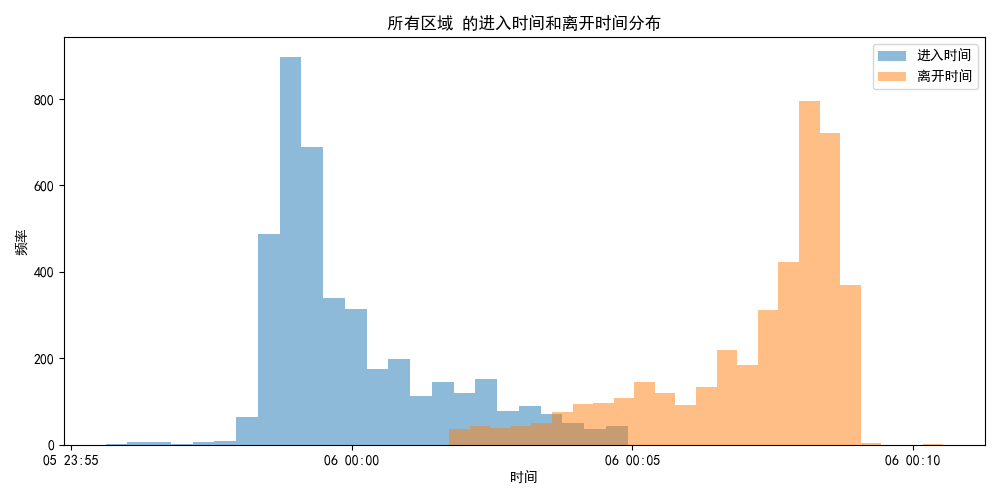
\includegraphics[width = \textwidth]{../img/时序分布/50万所有区域时间分布.png}
    \caption{所有区域进入时间和离开时间的分布,$n=500000$}
    \label{50}    
\end{figure}

\begin{figure}[htb]
    \centering
    \begin{subfigure}[b]{0.48\textwidth}
        \centering
        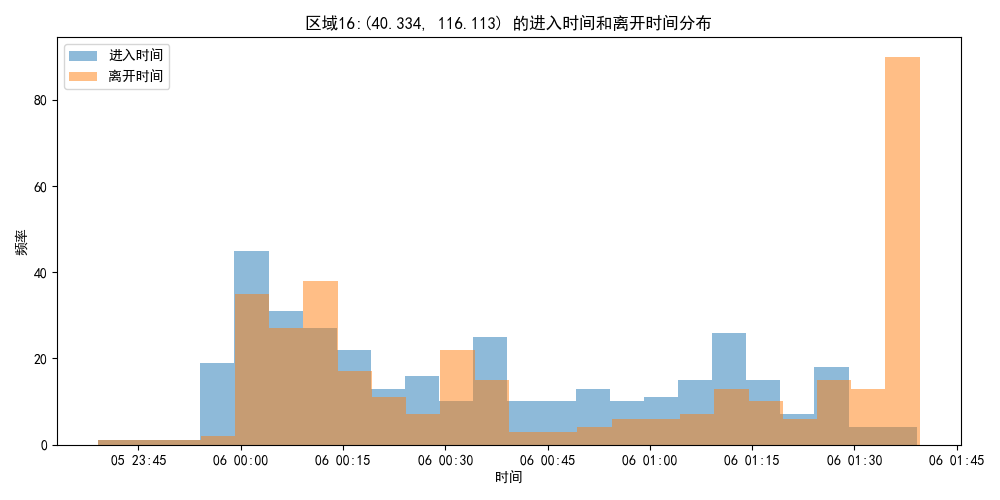
\includegraphics[width=\textwidth]{../img/时序分布/区域16时间分布.png}
        \caption{以区域16为例进入时间和离开时间的分布}
        \label{insimple}
    \end{subfigure}
    \hfill
    \begin{subfigure}[b]{0.48\textwidth}
        \centering
        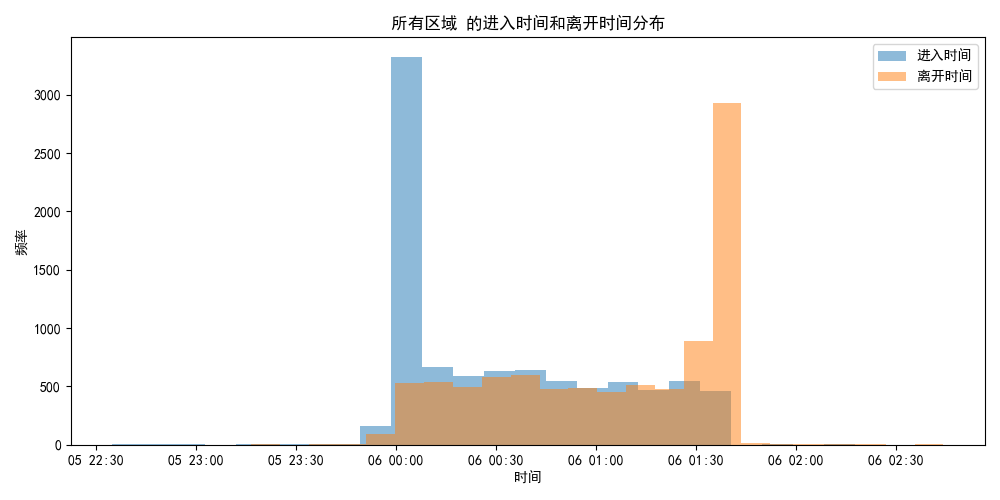
\includegraphics[width=\textwidth]{../img/时序分布/所有区域时间分布.png}
        \caption{前20名最密聚集地进入时间和离开时间的分布}
        \label{inall}
    \end{subfigure}
    \vfill
    \begin{subfigure}[b]{0.48\textwidth}
        \centering
        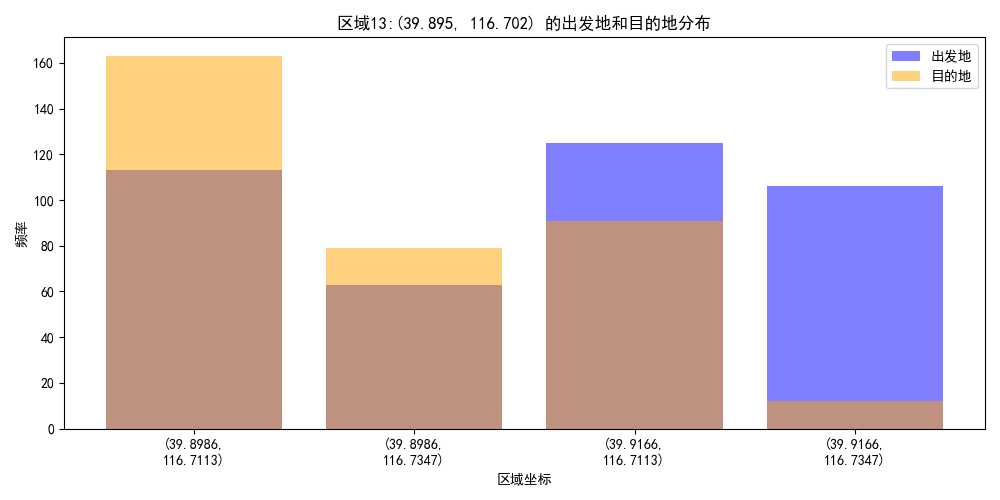
\includegraphics[width=\textwidth]{../img/OD分布/区域13出发地和目的地分布.png}
        \caption{以区域13为例目的地和出发地的分布}
        \label{odsimple}
    \end{subfigure}
    \hfill
    \begin{subfigure}[b]{0.48\textwidth}
        \centering
        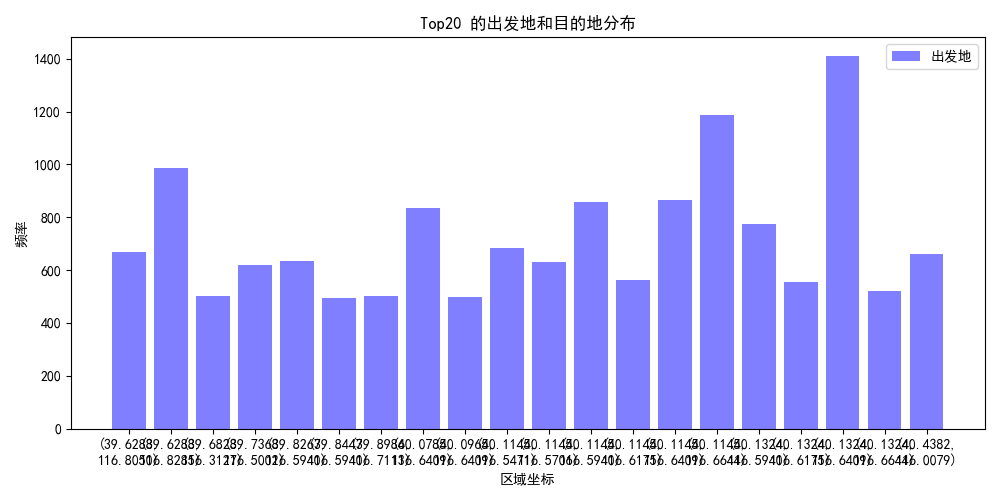
\includegraphics[width=\textwidth]{../img/OD分布/所有区域出发地和目的地分布.png}
        \caption{前20名最密聚集地目的地和出发地的分布}
        \label{odall}
    \end{subfigure}
    \caption{时间分布和OD分布}
    \label{fig:combined}
\end{figure}

\subsection{OD分析}

对于出发地和目的地,计算起来就更加复杂一些。这里我们假设出发地和目的地是某辆车到达计数区域或从计数区域出发后\textbf{连续静止}一段时间的一个区域。当车辆连续静止超过某个阈值时,我们就认为这是一个出发地或目的地。在实现上,仍然先根据车号分组,之后针对每一条有效的数据(也即\texttt{valid=True}),分别寻找其之前的若干条数据和之后的若干条数据,当这些数据的区域发生变化且连续静止时长超过阈值时进行统计即可。

关于阈值的选取,我们最终选取的阈值是$1200s$,也即当车辆在非当前区域的同一区域$S$存在两条静止记录,两条记录时间相差$1200s$以上,且这两条记录间的其他所有记录均在区域$S$中时,我们认为这是一个“目的地”或“聚集地”。这一方面考虑到我们的区域大小是$2km\times 2km$,对于一辆在行驶中的车辆来说,应当能够在$1200s$内穿越一个区域,另一方面是对于确实到达某一目的地或从某一出发地出发时,装卸货和行驶时间的和应当能够超过$1200s$。

不过最后的结果显示(图\ref{odmap}),这一方法并不理想,大部分目的地和出发地聚集在最密聚集地的周围,没能呈现出理想的结果。我们分析这可能是由于
\begin{itemize}[leftmargin=4em,itemsep=0pt,topsep=2pt]
    \item 车辆在到达某一聚集地前后可能需要加油、洗车等休整操作;
    \item 聚集地由于车辆聚集较多,更有可能出现交通堵塞、交通事故等情况,导致在聚集地附近的停留时间较长。
\end{itemize}

进一步调整阈值的过程中我们发现,阈值过大会导致目的地和出发地数据减少(满足前述条件的数据更少,可能由于车辆在静止状态下关闭了GPS等原因);阈值过小会导致目的地和出发地更加密集的向聚集地靠拢。这提示我们,或许在现有算法下仅依赖静止数据很难得出理想的结果。

\subsection{可视化结果}

我们分别针对每个聚集地,统计了目的地和出发地的分布(如图\ref{odsimple})、进入时间和离开时间的分布(如图\ref{insimple});以及所有20个聚集地的目的地和出发地分布(如图\ref{odall})、进入时间和离开时间的分布(如图\ref{inall})。这里仅展示部分内容,更多聚集地的统计结果可以在\texttt{./img/OD分析}中查看。


除此之外,我们还想知道这些位置到底在哪里,因此,我们把所有20个聚集地的目的地和出发地的前20名标注在了地图上(如图\ref{odmap})。针对这一结果的分析在上一小节,更加详细和全面的结果可以在\texttt{./html/Top20withOD.html}中查看。

\begin{figure}[htb]
    \centering
    \begin{minipage}{\textwidth}
        \centering
        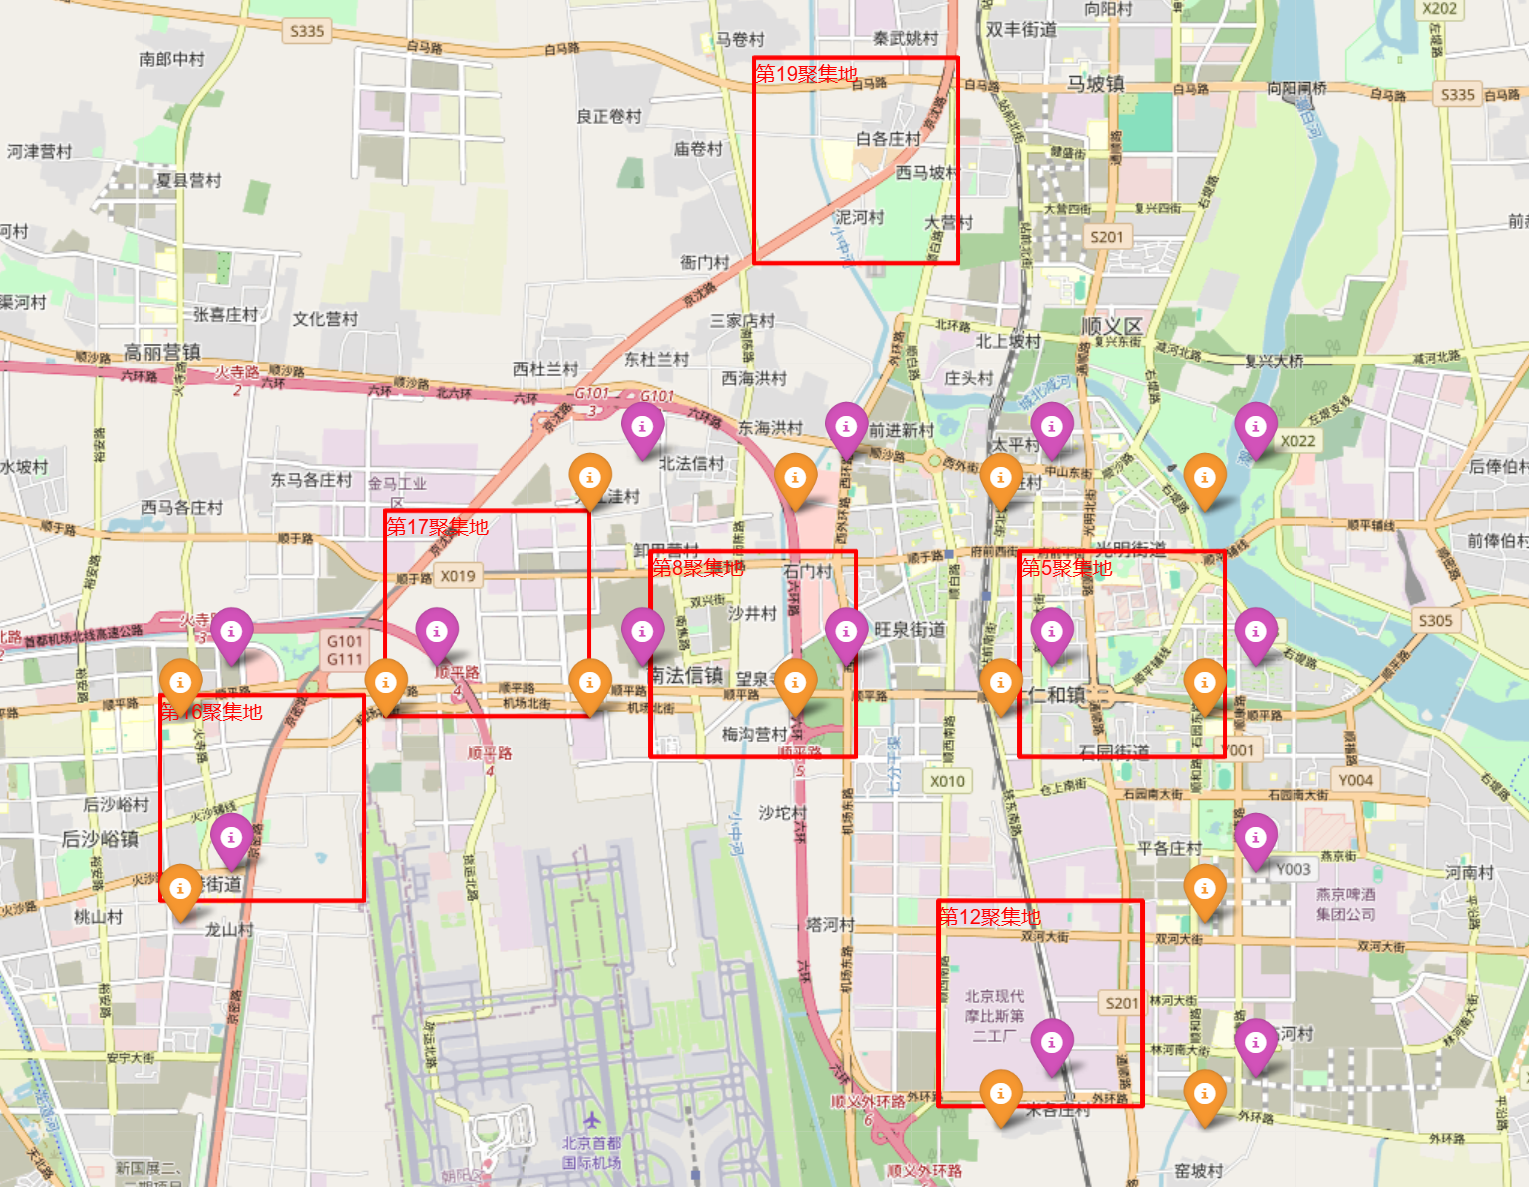
\includegraphics[width=\textwidth]{../img/聚集地和OD地图可视化.png}
        \caption{前20名最密聚集地和OD分布}
        \label{odmap}
    \end{minipage}
    \vspace{1em} % 添加垂直间距
    \begin{minipage}{\textwidth}
        \footnotesize % 调整注释文字大小
        \textbf{注:} 图中呈格点状分布,这是由于我们展示的是某个区域的左上角位置,因此不同区域的标记之间相差了整数个格长。
        \textbf{注:} 截取自\texttt{./html/Top20withOD.html}。 
    \end{minipage}
\end{figure}

\section{总结与反思}

在第三次作业的基础上,这次作业开展起来相对门槛较低。不过我仍然遇到了不小的问题。

首先由于算法和求解的问题更加复杂,代码的调试难度更大,当使用$500000$小样本时,时间长度的限制使得很难能检测出代码的问题,困扰很久后尝试将样本量增大大$500$万,部分问题才初见端倪。但受限于设备性能,此时代码运行速度大大降低。好在通过预先分析和控制算法复杂度没有出现内核崩溃或内存溢出的情况。

针对助教和老师的建议,我增加了针对聚集地结果的分析,但这些分析可能略显表面、仍有欠缺,如果能开展更多关于聚集地和聚集离开时间的分析会更好。

总的来讲,经过这次大作业的考验,我更加深刻的感受到了数据规模带来的挑战和机遇。数据中蕴藏着无尽的信息,如何从中提取有用的信息,是我们需要不断思考和探索的问题。但与此同时,信噪比较低的情况下,我们需要比较大量的样本才能够测试代码的可行性,因此我们需要不断提高代码效率,选取更加合适的采样方式等多种手段提升测试效率。

最后,感谢老师和助教一学期的辛苦付出!

\end{document}

